\documentclass[../Main.tex]{subfiles}

\begin{document}
\section{Basic Postulates of Relativity}
Maxwell's Equations, formulated by Maxwell in 1862, predict the existence of electromagnetic waves that travel at the speed of light. This is $c = 299792458 m s^{-1}$ (note that this number is precise, because it defines the metre).\par
A theory such as Maxwell's equations with a preferred velocity cannot be Galilean invariant. In principle this is permissible, sound waves travel through the air around $300 ms^{-1}$, but this is relative to the rest frame of the air. Thus, it was assumed that light must travel through a medium, this proposed medium was known as the Luminiferous Ether. However, experiments to demonstrate the existence of the Luminiferous Ether (Michelson \& Morley, 1881) showed that light travels at the same speed regardless of how fast the observer (on Earth) is moving through the Ether.\par
In 1905, Einstein postulated that there was no Ether. He provided two postulates:
\begin{enumerate}
    \item The laws of physics are the same in all inertial reference frames. This is the principle of relativity that Galileo postulated before.
    \item The speed of light in a vacuum is the same in all inertial reference frames. This is clearly not compatible with Galilean Relativity.
\end{enumerate}
\section{Lorentz Transformations in One Spatial Dimension}
\subsection{Deriving Lorentz Transformations}
We will derive the Lorentz transformations to replace Galilean transformations.\par
We will first consider 1 spatial dimension. An inertial frame $S$ has coordinates $(x, t)$. Consider a second frame $S'$ that moves at a speed $v$ relative to $S$ and has coordinates $(x', t')$.\par
According to Galileo, $x' = x - vt$ and $t' = t$.\par
This will not work, as the speed of light will not be constant in both frames. Instead consider a general transformation:
\begin{align*}
    x' &= f(x, t) \\
    t' &= g(x, t) \\
\end{align*}
Postulate 1 requires that in both frames $S$ and $S'$, a particle experiencing no forces must move at a constant velocity (Law of Inertia). So for a free particle in $S$, with $x = A + Bt$, the particle in $S'$ must be moving with $x' = A' + B't'$. Therefore the transformation $(f, g)$ must map lines in the $(x, t)$ plane to lines in the $(x', t')$ plane. Therefore $f$ and $g$ must be linear:
\begin{align*}
    x' &= ax + bt \\
    t' &= cx + dt
\end{align*}
Note that $a, b, c, d$ could depend on $v$ but must not depend on $x, t$. Note also that we have chosen the frames to have a common origin. We could just as well have added a constant term to both of the above equations.\par
The frame $S'$ is moving at speed $v$ in the frame $S$, but obviously must be at rest with respect to itself, $x' = 0$. Therefore the line $x = vt$ must be mapped to the line $x' = 0$. Therefore we can get the function $f$ up to scaling:
\begin{equation*}
    x' = \gamma_v (x - vt)
\end{equation*}
We can also relate in the other direction: $S$ moves at speed $-v$ in relation to $S'$, so $x = \gamma_{-v} (x' + vt)$.
\begin{proposition}
    In the above, $\gamma_v = \gamma_{-v}$
\end{proposition}
If we assume this to be true, we have that:
\begin{align}
    x' &= \gamma(x - vt) \label{eqnRelativePosGamma} \\
    t' &= \frac{1-\gamma^2}{\gamma v} x + \gamma t \label{eqnRelativeTimeGamma}
\end{align}
We cannot give a rigorous proof. We give 3 arguments:
\begin{enumerate}
    \item There is no preferred direction of space. Therefore $\gamma_v$ should be a function of $|v|$ only: $\gamma_v = \gamma_{-v}$.
    \item Consider frames $\tilde{S}$ and $\tilde{S'}$ where the $x$ axis is reflected. That is, $\tilde{x} = -x, \tilde{x'} = -x'$. Then if $S$ moves at speed $v$ with respect to $S'$, $\tilde{S}$ moves at speed $-v$ with respect to $\tilde{S'}$. Therefore
    \begin{align*}
        \tilde{x'} &= \gamma_{-v}(\tilde{x} + vt) \\
        -x' &= \gamma_{-v} (-x + vt) \\
        x' &= \gamma_{-v} (x - vt) \\
        \gamma_v &= \gamma_{-v}
    \end{align*}
    \item If a particle increases to speed $v$ relative to $S$, and then changes its speed by $-v$, it returns to rest is $S$. Consider the $x$ coordinate after these two changes in speed, assuming $\gamma_v = \gamma_{-v} = \gamma$:
        \begin{align*}
            x'' &= \gamma_{-v} (x' + vt') \\
            &= \gamma \left(\gamma (x - vt) + v\left(\gamma t + \frac{1 - \gamma^2}{\gamma v}\right)\right) \\
            &= x
        \end{align*}
\end{enumerate}
The final piece of information is postulate 2: the speed of light is the same in all frames. Therefore the light ray (path taken by light) $x = ct$ in $S$ must map to another light ray $x' = ct'$ under a Lorentz transformation.
\begin{align*}
    x' &= ct' \\
    \gamma (x - vt) &= c(\gamma t + \frac{1 - \gamma^2}{\gamma v}x) \\
    \gamma (c - v)t &= c(\gamma + \frac{1 - \gamma^2}{\gamma v}c)t \\
    \gamma (c - v) &= c(\gamma + \frac{1 - \gamma^2}{\gamma v}c)
\end{align*}
Then solving this final equation (a quadratic) for $\gamma$, the result is:
\begin{equation}
    \gamma = \frac{1}{\sqrt{1 - \frac{v^2}{c^2}}}
    \label{eqnLorentzFactor}
\end{equation}
Note that here we choose the positive root, since the negative root would correspond to a reflection in the axis.\par
Our equations \ref{eqnRelativePosGamma} and \ref{eqnRelativeTimeGamma} then become:
\begin{align}
    x' &= \gamma (x - vt) \label{eqnRelativePos} \\
    t' &= \gamma \left(t - \frac{v}{c^2}x\right) \label{eqnRelativeTime}
\end{align}
We can also check that in the case $v << c$ we recover Galilean Transformations: here we have $\gamma \approx 1$ and $\frac{v}{c} \approx 0$, and we do indeed get $x' = x - vt, t' = t$.
\subsection{Addition of Velocities}
We consider a particle moving with speed $u'$ in a frame $S'$, which in turn moves at speed $v$ in a frame $S$. We therefore consider what speed the particle moves in frame $S$.
\begin{equation*}
    u = \frac{x}{t}
\end{equation*}
We require the inverse Lorentz transformations. We have already argued that these are:
\begin{align*}
    x &= \gamma (x' + vt') \\
    t &= \gamma (t' + \frac{v}{c^2}x')
\end{align*}
\begin{align*}
    u &= \frac{x}{t} = \frac{\gamma(x' + vt')}{\gamma(t' + \frac{v}{c^2}x')} \\
    &= \frac{\frac{x'}{t'} + v}{1 + \frac{v}{c^2}\frac{x'}{t'}} \\
\end{align*}
\begin{equation}
    u = \frac{u' + v}{1 + \frac{vu'}{c^2}}
    \label{eqnAdditionVelocities}
\end{equation}
Again, note that this denominator is approximately 1 when $v$ and $u'$ are much smaller than $c$.
\begin{example}
    Consider, for example, $u' = v = \frac{c}{2}$. Then equation~\ref{eqnAdditionVelocities} gives that the added velocity is:
    \begin{equation*}
        u = \frac{c}{1 + \frac{1}{4}} = \frac{4}{5} c
    \end{equation*}
    Also, if one of the speeds is $c$: as in the case $v = c, u' = \frac{c}{d}$ where $d > 1$:
    \begin{align*}
        thing &= thing %TODO: Finish
    \end{align*}
\end{example}
Therefore, we cannot make something go faster than the speed of light by considering a frame moving towards it.
\subsection{Spacetime Diagrams and Simultaneity}
We introduce spacetime diagrams, an example of which is in figure~\ref{figSpacetimeDiagram}.
\begin{figure}[ht]
    \centering
    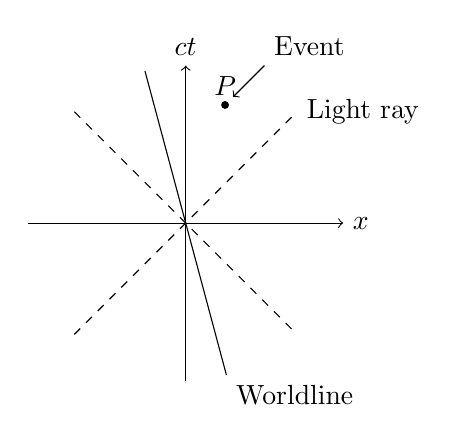
\begin{tikzpicture}
        \draw[->] (-2, 0) -- (2, 0) node[right] {$x$};
        \draw[->] (0, -2) -- (0, 2) node[above] {$ct$};

        \fill (0.5, 1.5) circle[radius=0.5mm];
        \node[anchor=south] at (0.5, 1.5) {$P$};

        \draw[->] (1, 2) node[anchor=south west] {Event} -- (0.6, 1.6);
        \draw[dashed] (225:2) -- (45:2) node[anchor=west] {Light ray};
        \draw[dashed] (135:2) -- (315:2);
        
        \draw (285:2) node[anchor=north west] {Worldline}
            -- (105:2);
    \end{tikzpicture}
    \caption{An example spacetime diagram}
    \label{figSpacetimeDiagram}
\end{figure}
We may put axes for a different frame $S'$ on the spacetime diagram of frame $S$. Let this move at speed $v$ relative to $S$. Then the $t'$ axis is when $x' = 0$, that is $ct = \frac{c}{v} x$. The $x'$ axis is at $t' = 0$, which is $ct = \frac{v}{c} x$. Figure~\ref{figSpacetimeDoubleAxis} shows what these new axes look like.
\begin{figure}[ht]
    \centering
    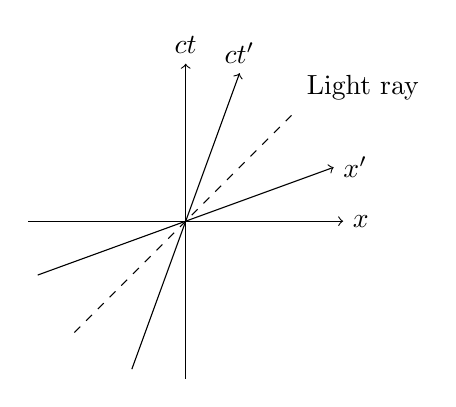
\begin{tikzpicture}
        \draw[->] (-2, 0) -- (2, 0) node[right] {$x$};
        \draw[->] (0, -2) -- (0, 2) node[above] {$ct$};
        \draw[->] (200:2) -- (20:2) node[right] {$x'$};
        \draw[->] (250:2) -- (70:2) node[above] {$ct'$};
        \draw[dashed] (225:2) -- (45:2) node[above right] {Light ray};
    \end{tikzpicture}
    \caption{Spacetime diagram with two sets of axes.}    
    \label{figSpacetimeDoubleAxis}
\end{figure}
Axes are always symmetric about the line $ct = x$, the path of a light ray.\par
We may also draw lines of constant $t$ or $t'$. These are horizontal in the frame $S$. Events that happen at the same time in the frame $S$ are \underline{simultaneous}. However, lines of constant $t'$ are not horizontal, so the same events (that are simultaneous in frame $S'$) are not simultaneous in the frame $S'$. If two events are separated in space and happen at the same time in $S$, they do not necessarily happen at the same time in a different frame $S'$.\par
This is the \underline{relativity of simultaneity}. This is an immediate consequence of the invariance of the speed of light.\par
\subsection{Causality and Light Cones}
Causality is the physical idea that causes must come before effects. If we have no simultaneity, is it therefore possible that causes could be seen after effects in some frame? This notion is solved by the fact that lines of simultaneity cannot make an angle of greater than $\frac{\pi}{4}$ because a frame can have relative velocity at most $c$ to another. This idea is made clearer by \underline{light cones}.
\begin{figure}[ht]
    \centering
    \begin{tikzpicture}[scale=2]
        \draw[->] (-0.5, 0) -- (2.1, 0) node[right] {$x$};
        \draw[->] (0, -0.5) -- (0, 2.1) node[above] {$ct$};

        \node[anchor=west] at (1, 1) {$P$};
        \fill (1, 1) circle[radius=0.2mm];
        \fill (1, 1.3) circle[radius=0.2mm];
        \node[anchor=west] at (1.5, 1.3) {$R$};
        \fill (1.5, 1.3) circle[radius=0.2mm];

        \draw[pattern=north east lines] (1, 1) -- (2, 2) -- (0, 2) -- cycle;
        \draw[pattern=north east lines] (0, 0) -- (2, 0) -- (1, 1) -- cycle;
        \node[anchor=west, shape=rectangle, fill=white, inner sep=0pt, outer sep=2pt] at (1, 1.3) {$Q$};
        \draw[->] (2, 1.5) node[anchor=west, align=left] {Future\\light cone}
            -- (1, 1.5);
        \draw[->] (2, 0.5) node[anchor=west, align=left] {Past\\light cone}
            -- (1, 0.5);
        
    \end{tikzpicture}
    \caption{Spacetime diagram with light cones}
    \label{figLightCones}
\end{figure}
Then, in figure~\ref{figLightCones}, $Q$ could be caused by $P$, but $R$ could not be caused by $P$ since it is outside the future light cone. $P$ can be caused by any event inside the past light cone.\par
Given a second frame $S'$, the lines of constant $t'$ must make an angle less than $\frac{\pi}{4}$ to the horizontal. Thus, in figure~\ref{figLightCones}, we can find a frame in which $P$ and $R$ are simultaneous, but there can be no frame in which $P$ and $Q$ are simultaneous. The future light cone for $P$ is always to the future of $P$, in any frame.\par
Because nothing travels faster than light, this is sufficient to ensure causality. That is, all frames agree on what can influence what: events can only influence other events in the future light cone.
\subsection{Time Dilation}
Consider a clock at rest in a frame $S'$. This ticks at intervals $T'$. Then we consider each clock tick as an event. Each event $P_i$ happens at coordinates $(c(t'_0 + iT), 0)$. We then use the inverse Lorentz transformation to return to a frame $S$ and consider when the events $P_i$ happen:
\begin{equation*}
    t = \gamma(t' + \frac{vx'}{c^2})
\end{equation*}
Given that $x' = 0$, $t = \gamma t'$.\par
Therefore, the period between ticks in frame $S$ is $T = \gamma T'$. Recall that $\gamma \geq 1$, and so $T \geq T'$. That is, moving clocks run slow.
\begin{example}[Twin Paradox]
    Consider two twins (with the same age). Suppose that twin $A$ stays on earth, and twin $B$ travels towards Neptune and back at speed close to $c$.\par
    Then twin $A$ sees twin $B$'s clock tick more slowly and therefore $A$ expects $B$ to be younger when they return.\par
    However, from the point of view of twin $B$, the Earth is travelling away from them at speed close to $c$ and so clocks on Earth appear to tick slower. Therefore, it would appear that twin $A$ would be younger.\par
    The paradox is broken because twin $B$ has to turn around to get back.\par
    From the perspective of twin $A$, a time $2T$ has passed. As we have seen, $2T' = \frac{2T}{\gamma}$ has passed for $B$.\par
    For $B$, while travelling away $A$'s clock ticks more slowly, and also while coming back: $2T = \frac{2T'}{\gamma}$. However, this accounting misses the jump in velocity (and thus lines of simultaneity) when $B$ turns around. When this time is added back in, the times agree again. This is seen in Example Sheet 4.
\end{example}
\begin{figure}[ht]
    \centering
    \begin{tikzpicture}[scale=2]
        \draw[->] (0, 0) -- (2.1, 0) node[right] {$x$};
        \draw[->] (0, 0) -- (0, 3.1) node[above] {$ct$};

        \draw (0, 0) -- (0.7, 1.5)
            node[anchor=north west, pos=0.5] {$B$} -- (0, 3);
        \draw[dashed] (0.7, 0) -- (0.7, 3) node[above] {Neptune};

        \node[anchor=east] at (0, 0.7) {$A$};

        \draw (0, 1.5) -- (1, 1.5) node[right, align=left] {Line of simultaneity\\for $A$};

        \draw[dashed] (0, 2) -- (1.5, 0.93);

    \end{tikzpicture}
    \caption{Spacetime diagram for twin paradox}
    \label{figTwinParadox}
\end{figure}
\subsection{Length Contraction}
Consider a rod that has length $L'$, at rest in a frame $S'$.
\begin{figure}[ht]
    \centering
    \begin{tikzpicture}
        \draw (0, 0) -- (2.1, 0) node[right] {$x'$};
        \draw (0, 0) -- (0, 2.1) node[above] {$ct'$};
    \end{tikzpicture}
    \caption{Spacetime diagram for length contraction}
    \label{figLengthContraction}
\end{figure}
We define length to be the distance between endpoints at equal times.\par
Then in a frame $S$, the rod has length $L$. Then, as seen in figure~\ref{figLengthContraction}, the events of the two ends of the rod at time $t' = 0$ are not simultaneous in $S$. In fact, we have that:
\begin{align*}
    P_1 &= (0, 0) \text{ in both frames} \\
    P_2 &= (0, L') \text{ in frame } S' \\
    P_2 &= \left(\gamma \frac{v}{c} L', \gamma L'\right) \text{ in frame } S
\end{align*}
Now note that $S'$ is moving at speed $v$ relative to $S$, so $P_3$ has x-coordinate:
\begin{align*}
    x &= \gamma L' - vt \\
    &= \gamma L' - \frac{\gamma v L'}{c^2} \\
    &= \gamma(1 - \frac{v^2}{c^2}) L' \\
    &= \frac{L'}{\gamma}
\end{align*}
So the new length is $L = \frac{L'}{\gamma}$. This is called Lorentz contraction
\begin{example}[Ladder and Barn thought experiment]
    Imagine a ladder has length $2L$ and a barn has length $L$ with open doors on both sides. Suppose that the ladder moves at a speed such that $\gamma = 2$. Lorentz contraction therefore implies that, in the frame of the barn, the ladder has length $L$ and fits in the barn. However, in the frame of the ladder the barn is contracted and the ladder is four times too long.
\end{example}
\section{Preserved Quantities in One Spatial Dimension}
\subsection{The Invariant Interval}
\begin{definition}{Invariant interval}
    Consider two events $P_1$ and $P_2$ with coordinates $(ct_1, x_1)$ and $(ct_2, x_2)$ in frame $S$. Define:
    \begin{align*}
        \Delta t &= t_2 - t_1 \\
        \Delta x &= x_2 - x_1
    \end{align*}
    Then the \underline{invariant interval} is:
    \begin{equation}
        (\Delta s)^2 = c^2(\Delta t)^2 - (\Delta x)^2
        \label{eqnInvariantInterval}
    \end{equation}
\end{definition}
We show that this is invariant. Consider the same points in the frame $S'$:
\begin{align*}
    (\Delta s')^2 &= c^2(\Delta t')^2 - (\Delta x')^2 \\
    &= \gamma^2\left(c\Delta t - \frac{v}{c} \Delta x\right)^2 - \gamma^2 \left(\Delta x - v \Delta t\right)^2 \\
    &= \gamma^2\left(c^2 - v^2\right)\left(\Delta t\right)^2 - \gamma^2 \left(1 - \frac{v^2}{c^2}\right)^2 \left(\Delta x\right)^2 \\
    &= c^2 (\Delta t)^2 - (\Delta x)^2 \\
    &= (\Delta s)^2
\end{align*}
So the invariant interval is indeed invariant. Note that we can also write:
\begin{equation}
    (\Delta s)^2 = \begin{pmatrix}c\Delta t & \Delta x\end{pmatrix} \begin{pmatrix}1 & 0 \\ 0 & -1\end{pmatrix} \begin{pmatrix} c\Delta t \\ \Delta x\end{pmatrix}
    \label{eqnMinkowskiMetric}
\end{equation}
The matrix is known as the \underline{Minkowski metric}.\par
We can also write the Lorentz Transformations in this way:
\begin{equation}
    \begin{pmatrix} ct' \\ x'\end{pmatrix} = \begin{pmatrix}\gamma & -\frac{\gamma v}{c} \\ -\frac{\gamma v}{c} & \gamma\end{pmatrix} \begin{pmatrix}ct \\ x\end{pmatrix}
    \label{eqnLorentzMatrices}
\end{equation}
Note that the statement that $(\Delta s)^2$ is invariant is equivalent to the statement that:
\begin{equation}
    \begin{pmatrix}\gamma & -\frac{\gamma v}{c} \\ -\frac{\gamma v}{c} & \gamma\end{pmatrix} \begin{pmatrix} 1 & 0 \\ 0 & -1\end{pmatrix}\begin{pmatrix}\gamma & -\frac{\gamma v}{c} \\ -\frac{\gamma v}{c} & \gamma\end{pmatrix} = \begin{pmatrix}1 & 0 \\ 0 & -1\end{pmatrix}
    \label{eqnLorentzPreserveMinkowski}
\end{equation}
That is, Lorentz transformations preserve the Minkowski metric under conjugation. Note that the Minkowski metric is not positive-definite: 

\begin{tabular}{c|c}
    Sign of $(\Delta s)^2$ & Name \\
    \hline
    $(\Delta s)^2 > 0$ & Time-like separated \\
    $(\Delta s)^2 < 0$ & Space-like separated \\
    $(\Delta s)^2 = 0$ & Light-like separated \\
\end{tabular}

In particular, two points with $(\Delta s)^2 = 0$ are connected-by a light ray.
\begin{figure}[ht]
    \centering
    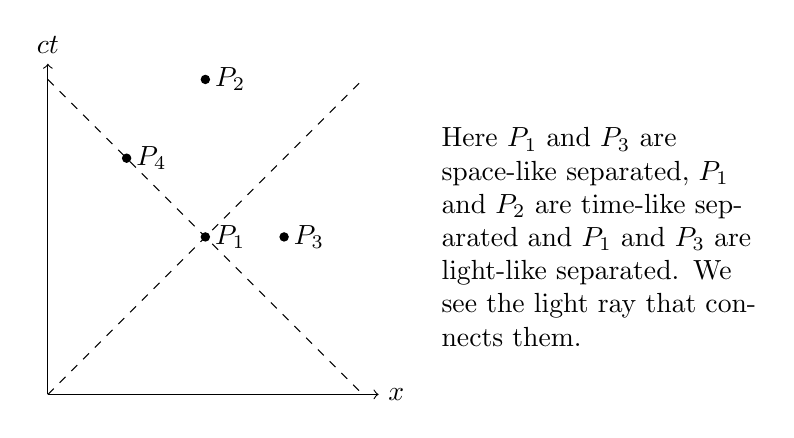
\begin{tikzpicture}[scale=2]
        \draw [->] (0, 0) -- (2.1, 0) node[right] {$x$};
        \draw [->] (0, 0) -- (0, 2.1) node[above] {$ct$};

        \draw[dashed] (0, 0) -- (2, 2);
        \draw[dashed] (0, 2) -- (2, 0);

        \fill (1, 1) circle[radius=0.3mm] node[right] {$P_1$};
        \fill (1, 2) circle[radius=0.3mm] node[right] {$P_2$};
        \fill (1.5, 1) circle[radius=0.3mm] node[right] {$P_3$};
        \fill (0.5, 1.5) circle[radius=0.3mm] node[right] {$P_4$};

        \node[text width=4cm] at (3.5, 1) {Here $P_1$ and $P_3$ are space-like separated, $P_1$ and $P_2$ are time-like separated and $P_1$ and $P_3$ are light-like separated. We see the light ray that connects them.};

    \end{tikzpicture}
    \caption{Spacetime diagram of different events and separations}
    \label{figSpaceTimeSeparations}
\end{figure}
\subsection{Rapidity}
We have seen that, as rotations preserve length, Lorentz transformations preserve the Minkowski Metric. To make this clearer, we can define:
\begin{definition}{Rapidity}
    For a given Lorentz transformation, with Lorentz factor $\gamma$, the \underline{rapidity}, $\phi$, is:
    \begin{equation*}
        \gamma = \cosh(\phi)
    \end{equation*}
    Note that this gives $\sinh(\phi) = \frac{\gamma v}{c}$.
\end{definition}
We can then re-write the Lorentz transformation matrix using rapidity:
\begin{equation}
    \Lambda(\phi) =
    \begin{pmatrix}
        \cosh(\phi) & -\sinh(\phi) \\
        -\sinh(\phi) & \cosh(\phi)
    \end{pmatrix}
    \label{eqnRapidityMatrix}
\end{equation}
We can check also that the application of two Lorentz transformations adds rapidity:
\begin{equation*}
    \Lambda(\phi_1) \Lambda(\phi_2) = \Lambda(\phi_1 + \phi_2)
\end{equation*}
Note that this does not apply for velocities. See earlier, where we derived that the new velocity is $\frac{v_1 + v_2}{1 + \frac{v_1}{v_2}{c^2}}$.
\section{Lorentz Transformations in Three Spatial Dimensions}
We will now consider a similar approach (via conserved quantities) to describe Lorentz transformations in 4 dimensions - 3 spatial dimensions and 1 time dimension. The 4-dimensional Minkowski metric is:
\begin{equation*}
    \eta = 
    \begin{pmatrix}
        1&0&0&0\\
        0&-1&0&0\\
        0&0&-1&0\\
        0&0&0&-1
    \end{pmatrix}
\end{equation*}
\begin{remark}
    If indices are needed to be used, often Greek letters are used to denote this, e.g. $\eta_{\mu \nu}$.
\end{remark}
An event in spacetime is given by a 4-vector:
\begin{equation*}
    X = (ct, x, y, z)
\end{equation*}
We will use capital letters and no bold text for 4-vectors. We will write indices above the vector, like $X^\mu$, and again use Greek letters.

The invariant distance between $X$ and the origin is given by:
\begin{align*}
    X \cdot X &= X^T \eta X \\
    &= c^2 t^2 - x^2 - y^2 - z^2
\end{align*}
Note that in index notation this would be $X^\mu \eta_{\mu \nu} X^\nu$

This is a pseudo-inner product, since $X \cdot X$ is not necessarily positive. It is, however, the inner product we will use.
As in 2 dimensions, we have ideas of light-like and spacelike: if $X \cdot X > 0$ then $X$ is time-like, and if it is negative then $X$ is space-like. If $X \cdot X = 0$, then $X$ is light-like, also known as null.
\subsection{Matrix Representation of Lorentz Transformations}
Lorentz transformations are $4\times 4$ matrices $\Lambda$ such that $X' = \Lambda X$. The defining feature of Lorentz transformations is that they leave the inner product invariant for all $X$:
\begin{equation*}
    X'\cdot X' = X \cdot X
\end{equation*}
This is only possible if $\Lambda$ preserves the Minkowski metric:
\begin{equation}
    \Lambda^T \eta \Lambda = \eta
    \label{eqnLorentzPreserveMinkowski4}
\end{equation}
We can then derive what matrices $\Lambda$ are possible. By equation~\ref{eqnLorentzPreserveMinkowski4}, $\Lambda$ must be symmetric. Therefore there are only 10 constraints on $\Lambda$, and so we can find 6 independent transformations for $\Lambda$.
3 of them are rotations, since these preserve both the Euclidean and Minkowski metrics. If $R$ is a $3\times 3$ rotation matrix, then these have the form:
\begin{equation*}
    \Lambda =
    \begin{pmatrix}
        1 & 0 & 0 & 0 \\
        0 &   &   &   \\
        0 &   & \text{\Large R} &   \\
        0 &   &   &   \\
    \end{pmatrix}
\end{equation*}
Then the other 3 are Lorentz boosts in the $x$, $y$ and $z$ dimensions. The boost in the $X$ dimension is:
\begin{equation*}
    \Lambda =
    \begin{pmatrix}
        \gamma & -\frac{\gamma v}{c} & 0 & 0 \\
        -\frac{\gamma v}{c} & \gamma & 0 & 0 \\
        0 & 0 & 1 & 0 \\
        0 & 0 & 0 & 1
    \end{pmatrix}
\end{equation*}
\begin{definition}{Lorentz Group}
    The \underline{Lorentz group} in $(3+1)$-space consists of all $4\times 4$ matrices generated by the rotations and boosts about the axes, as seen above.
    It is denoted $O(1, 3)$.
\end{definition}
Because the inner product is preserved by these transformations, it is automatic that the speed of light is the same in all frames, because a null vector $X$ is preserved.
\begin{definition}{Proper Lorentz Group}
    The \underline{proper Lorentz group} is defined to be $SO(1, 3)$: all the matrices of $O(1, 3)$ that have determinant 1.
\end{definition}
However, there still exist some matrices in $SO(1, 3)$ that change the direction of time. In order to exclude these we define:
\begin{definition}{Proper orthochronous Lorentz group}
    The \underline{proper orthochronous Lorentz group} is all matrices in $SO(1, 3)$ that preserve the direction of time. It is denoted $SO^+(1, 3)$.
\end{definition}
For example, the matrix:
\begin{equation*}
    \begin{pmatrix}
        -1 & 0 & 0 & 0 \\
        0 & -1 & 0 & 0 \\
        0 & 0 & -1 & 0 \\
        0 & 0 & 0 & -1
    \end{pmatrix}
\end{equation*}
flips the direction of time so is not in $SO^+(1, 3)$.
From now on we will consider Lorentz transformations to be those in $SO^+(1, 3)$.
\subsection{Proper Time}
In order to define ideas such as Newton's Second Law, we need to create new concepts of time and velocity that transform nicely under Lorentz transformations. To do this, we need to find a concept of time $\tau$ that is invariant under Lorentz transformations. Then we would be able to define a concept of velocity:
\begin{equation*}
    U = \frac{dX}{d\tau}
\end{equation*}
\begin{definition}{Proper Time}
    Given two points along a worldline (line of motion of a particle inside a light cone), the invariant interval $\Delta s$ is the same in all inertial frames. Then define the \underline{proper time} elapsed between these two points to be:
    \begin{equation*}
        \Delta \tau = \frac{\Delta s}{c}
    \end{equation*}
\end{definition}
\begin{remark}
    As we wanted, all of these quantities are invariant in any frame and therefore so is $\Delta \tau$.
\end{remark}
For any given worldline, this can be parameterised by $\tau$, which all observers will agree on.

Along a small segment of the worldline,
\begin{align*}
    d\tau &= \frac{\sqrt{c^2 (dt)^2 - (d\vec{x})^2}}{c^2} \\
    &= dt \sqrt{1 - \left(\frac{d\vec{x}}{c dt}\right)^2}
\end{align*}
Then if we define $\vec{u} = \frac{d\vec{x}}{dt}$ to be the instantaneous 3-velocity of the particle in frame $S$,
\begin{equation*}
    d\tau = dt\sqrt{1 - \frac{\vec{u}^2}{c^2}}
\end{equation*}
Now, if we let $\gamma = \left(1-\frac{u^2}{c^2}\right)^{-\frac{1}{2}}$ (note that this is the same form as for the Lorentz factor, but we use the instantaneous 3-velocity, not the velocity of a moving frame),
\begin{equation}
    d\tau = \frac{dt}{\gamma}
    \label{eqnProperTime}
\end{equation}
Note also that $\gamma$ need not be constant, since the velocity of the particle could be changing. A clock following the worldline has $dx' = 0$, and therefore $d\tau = dt'$. That is, the proper time is the time measured by an observer following the worldline. The frame of this observer need not be inertial. To resolve the issue of a non-inertial frame, we consider instead a sequence of inertial frames, which the observer spends an infinitesimal time in. These frames follow the velocity $\vec{u}(t)$ at each instant in time.
\subsection{4-Velocity}
Now we have found an invariant $\tau$, and the 4-vector $X = (ct(\tau), x(\tau), y(\tau), z(\tau))$ transforms as $X' = \Lambda X$, the vector:
\begin{equation*}
    U = \frac{dX}{d\tau}
\end{equation*}
transforms as $U' = \Lambda U$. This in fact can be used to define a 4-vector: any vector that transforms in the way $V' = \Lambda V$.
We define this to be the 4-velocity:
\begin{definition}{4-velocity}
    For a particle with position 4-vector $X$, the \underline{4-velocity} is given by:
    \begin{equation*}
        U = \frac{dX}{d\tau}
    \end{equation*}
\end{definition}
We can find an explicit formula:
\begin{align*}
    U &= \frac{dX}{d\tau} = \begin{pmatrix}c\frac{dt}{d\tau} \\ \frac{d\vec{x}}{d\tau}\end{pmatrix} \\
    &= \frac{dt}{d\tau} \begin{pmatrix}c \\ \frac{d\vec{x}}{dt}\end{pmatrix} \\
    &= \gamma \begin{pmatrix}c \\ \vec{u} \end{pmatrix}
\end{align*}
Because $U$ is a 4-vector, its dot product must be the same in all frames:
\begin{align*}
    U \cdot U &= \gamma^2 c^2 - \gamma^2 \vec{u} \cdot \vec{u} \\
    &= \gamma^2 (c^2 - \vec{u} \cdot \vec{u}) \\
    &= \gamma^2 \frac{c^2}{\gamma^2} \\
    &= c^2
\end{align*}
This means that the 4-velocity is determined by the 3-velocity $\vec{u}$. That is, given a 4-velocity, we can solve for the time component of $U$.
\subsection{4-Momentum}
Now we have 4-velocity, it is easy to define the 4-momentum:
\begin{definition}{4-momentum and Relativistic Energy}
    Given a particle of rest mass $m$ and 4-velocity $U$, the \underline{4-momentum} is the product:
    \begin{equation*}
        P = mU
    \end{equation*}
\end{definition}
The rest mass is a scalar property of all particles.

Relativistic 3-momentum $\vec{p}$ is given by $\vec{p} = m\gamma \vec{u}$.
\begin{definition}{Relativistic energy}
    For a particle of rest mass $m$ and instantaneous Lorentz Factor $\gamma$, the \underline{relativistic energy} $E$ is:
    \begin{equation*}
        E = m\gamma c^2
    \end{equation*}
\end{definition}
Then the 4-momentum can be written as:
\begin{equation*}
    P = \begin{pmatrix}\frac{E}{c} \\ \vec{p} \end{pmatrix}
\end{equation*}
This 4-vector combines energy and 3-momentum in the same way that 4-velocity combined 3-velocity and proper time. In the absence of forces, the Lorentz-invariant generalisation of Newton's Second Law is:
\begin{equation}
    \frac{dP}{d\tau} = 0
    \label{eqnNewtonIIRelativity}
\end{equation}
This equation combines both conservation of momentum and conservation of energy. This cannot be derived, it must be taken as a new postulate. However, it is the best generalisation since in the limit $v << c$ we recover Newton's Second Law.

From $U \cdot U = c^2$ we get that $P \cdot P = m^2 c^2$, and we can also work out $P \cdot P$:
\begin{align*}
    P \cdot P &= \frac{E^2}{c^2} - \vec{p}^2 \\
    \therefore E^2 &= \vec{p}^2 c^2 + m^2 c^4
\end{align*}

Taking the non-relativistic limit:
\begin{align*}
    E &= m\gamma c^2 = \frac{mc^2}{\sqrt{1 - \frac{\vec{u}^2}{c^2}}} \\
    &\approx mc^2 \left[1 + \frac{1}{2} \frac{\vec{u}^2}{c^2} + \cdots \right] \\
    &= mc^2 + \frac{1}{2} m\vec{u}^2
\end{align*}
So we have a new consequence of relativity: an extra energy exists in the form of the \underline{rest mass energy}: $E_0 = mc^2$.

The quantity $\gamma m$ is sometimes called the \underline{relativistic mass}. This quantity is equal to $m$ when the object is at rest, but tends to $\infty$ as the particle reaches close to the speed of light. This can be thought of as the particle getting heavier, and needing more force to accelerate it. In particular, a finite force cannot accelerate a particle beyond the speed of light. We will see this in more detail later when forces are discussed. This also suggests that a particle with a non-zero mass must have speed less than $c$.
\subsection{Massless Particles}
In Galilean physics, the notion of a massless particle makes no sense because the momentum would vanish, and we could not write down Newton's Second Law. However, this idea does make sense for relativistic particles.

The product $P \cdot P = m^2 c^2$, so this suggests we can write $m = 0$:
\begin{equation}
    P \cdot P = 0.
    \label{eqnNullMomentum}
\end{equation}
That is, the 4-momentum of a massless particle is null, and lies along a light ray.

The 4-velocity does not exist for a massless particle, but the 4-momentum is the fundamental quantity, and does exist. From equation~\ref{eqnNullMomentum}, a massless particle has:
\begin{equation*}
    P = \frac{E}{c}\begin{pmatrix}1 & \uvec{n}\end{pmatrix}
\end{equation*}
This obeys the required equation. Here $E$ will be the energy of the massless particle. It is not equal to $m \gamma c^2$, since this is for massive particles only. We may then define the 3-momentum $\vec{p} = \frac{E}{c} \uvec{n}$.

We can interpret a 3-velocity: $\vec{u} = c\uvec{n}$, and we therefore have $\vec{u}^2 = c^2$ and so the massless particle travels at the speed of light. We then have $|\vec{u}| = 0$ is and only if the particle is massless.

Along a light-ray, $d\tau = 0$ since the points are light-like separated. Therefore, no time passes in the frame of the massless particle.

Only two massless particles are known. These are the photon (the exchange particle for light) and the theorised graviton (which is the exchange particle for gravity). We borrow from quantum mechanics that the energy of a photon is related to its frequency: $E = \hbar \omega = \hbar \frac{2\pi c}{\lambda}$.
\end{document}